You will use the piezoelectric disc to generate the required tones.

\subsection{Theory of Operation}

Piezoelectric crystals have a property that causes them to turn mechanical energy into electrical energy, and vice-versa.
I'm pretty sure the piezodiscs were included in the ``common kit'' so that electrical engineering students could design a transistor-based amplifying circuit and then use the piezodiscs as ``force sensors.''

We will drive the piezodiscs in the other direction: we will apply electricity to the crystal to cause the brass plate to deform, and then remove the electricity to allow the brass plate to relax.
By repeatedly doing this, we will cause the piezodisc to produce sound.
Normally when used to generate sound, the device would be enclosed in a resonating chamber to increase the sound's volume;
for the benefit of everyone's ears, perhaps it is best that we won't have a lab room full of loud audio devices.

The specification calls for a 5kHz tone.
This means that the audio wave must reach its peak 5,000 times per second.
Put another way, during every second there must be 5,000 peaks -- dividing that out, we see that there must be 200\textmu s between the wave's peaks.

\subsection{Practical Considerations}

The piezodiscs have enough internal resistance that we can safely drive the crystal directly from an Arduino pin.

As we will be driving the piezodisc with a digital output pin, we cannot produce a pure sine wave;
instead we will produce a square wave.
Because it will be a square wave, in addition to the 5kHz tone, there will also be a 15kHz harmonic, plus other harmonics beyond the range of human hearing.
We will not attempt to suppress the harmonics.

To produce the exact 5kHz square wave, you need to use a timer interrupt.
At first glance, you might think to generate an interrupt every 200\textmu s;
however, the wave needs to have a peak \textit{and} a trough every 200\textmu s.
(Without troughs, there are no peaks.)
Therefore, you want to generate an interrupt every 100\textmu s, alternatingly setting the Arduino pin logic-high and logic-low.

\subsection{Examining the Starter Code}

The \function{initialize_alarm()} function is where you'll place any alarm-related code that needs to be run once when the program starts.
The \function{manage_alarm()} function is where you'll place any alarm-related code that needs to run with every iteration of the program's main loop.
You will, of course, add code outside these functions too: an interrupt service routine for a timer, and possibly helper functions.

You'll also notice two variables in the starter code.
The \lstinline{on_period} variable will be used to control how long a tone is generated and the LEDs are illuminated when in Single Pulse mode and when in Normal Operation mode.
The \lstinline{total_period} variable will be used to control the time between alarms when in Normal Operation mode.

\subsection{Continuous Tone}

Using the ``Timers'' section of the Cow Pi datasheet,\footnote{
    \url{https://cow-pi.readthedocs.io/en/latest/microcontroller.html\#timers}
}
place code in \function{initialize_alarm()} to configure Timer2 to produce a comparison interrupt every 100\textmu s, using the ``Clear Timer on Compare'' mode.
Also place in \function{initialize_alarm()} code to enable that interrupt.

Use the \function{ISR} macro to create an interrupt service routine in \textit{alarm.c} for that interrupt.
In that ISR, add code so that on every other invocation will place a 1 on Arduino pin D13 and will place a 0 on the alternate invocations.

Test that your code is generating a tone on the piezodisc, and correct any errors.

After you have code that generates a tone, test that it generates a 5kHz tone.
In a web browser, load the Husker~Scope Spectrum Analyzer.\footnote{
    \url{https://cse.unl.edu/~jfalkinburg/husker-scope/app/page/SpectrumAnalyzer}
}
Place your Cow Pi near your computer's microphone.
While the piezodisc is producing a tone, click on the ``Auto'' button in the control-cluster on the right-side of Husker~Scope.
Husker~Scope should then display something similar to Figure~\ref{fig:spectrumAnalyzer}.
Confirm that the center frequency on the display is at or very near 5,000Hz.
Correct any errors.

\begin{figure}
    \centering
    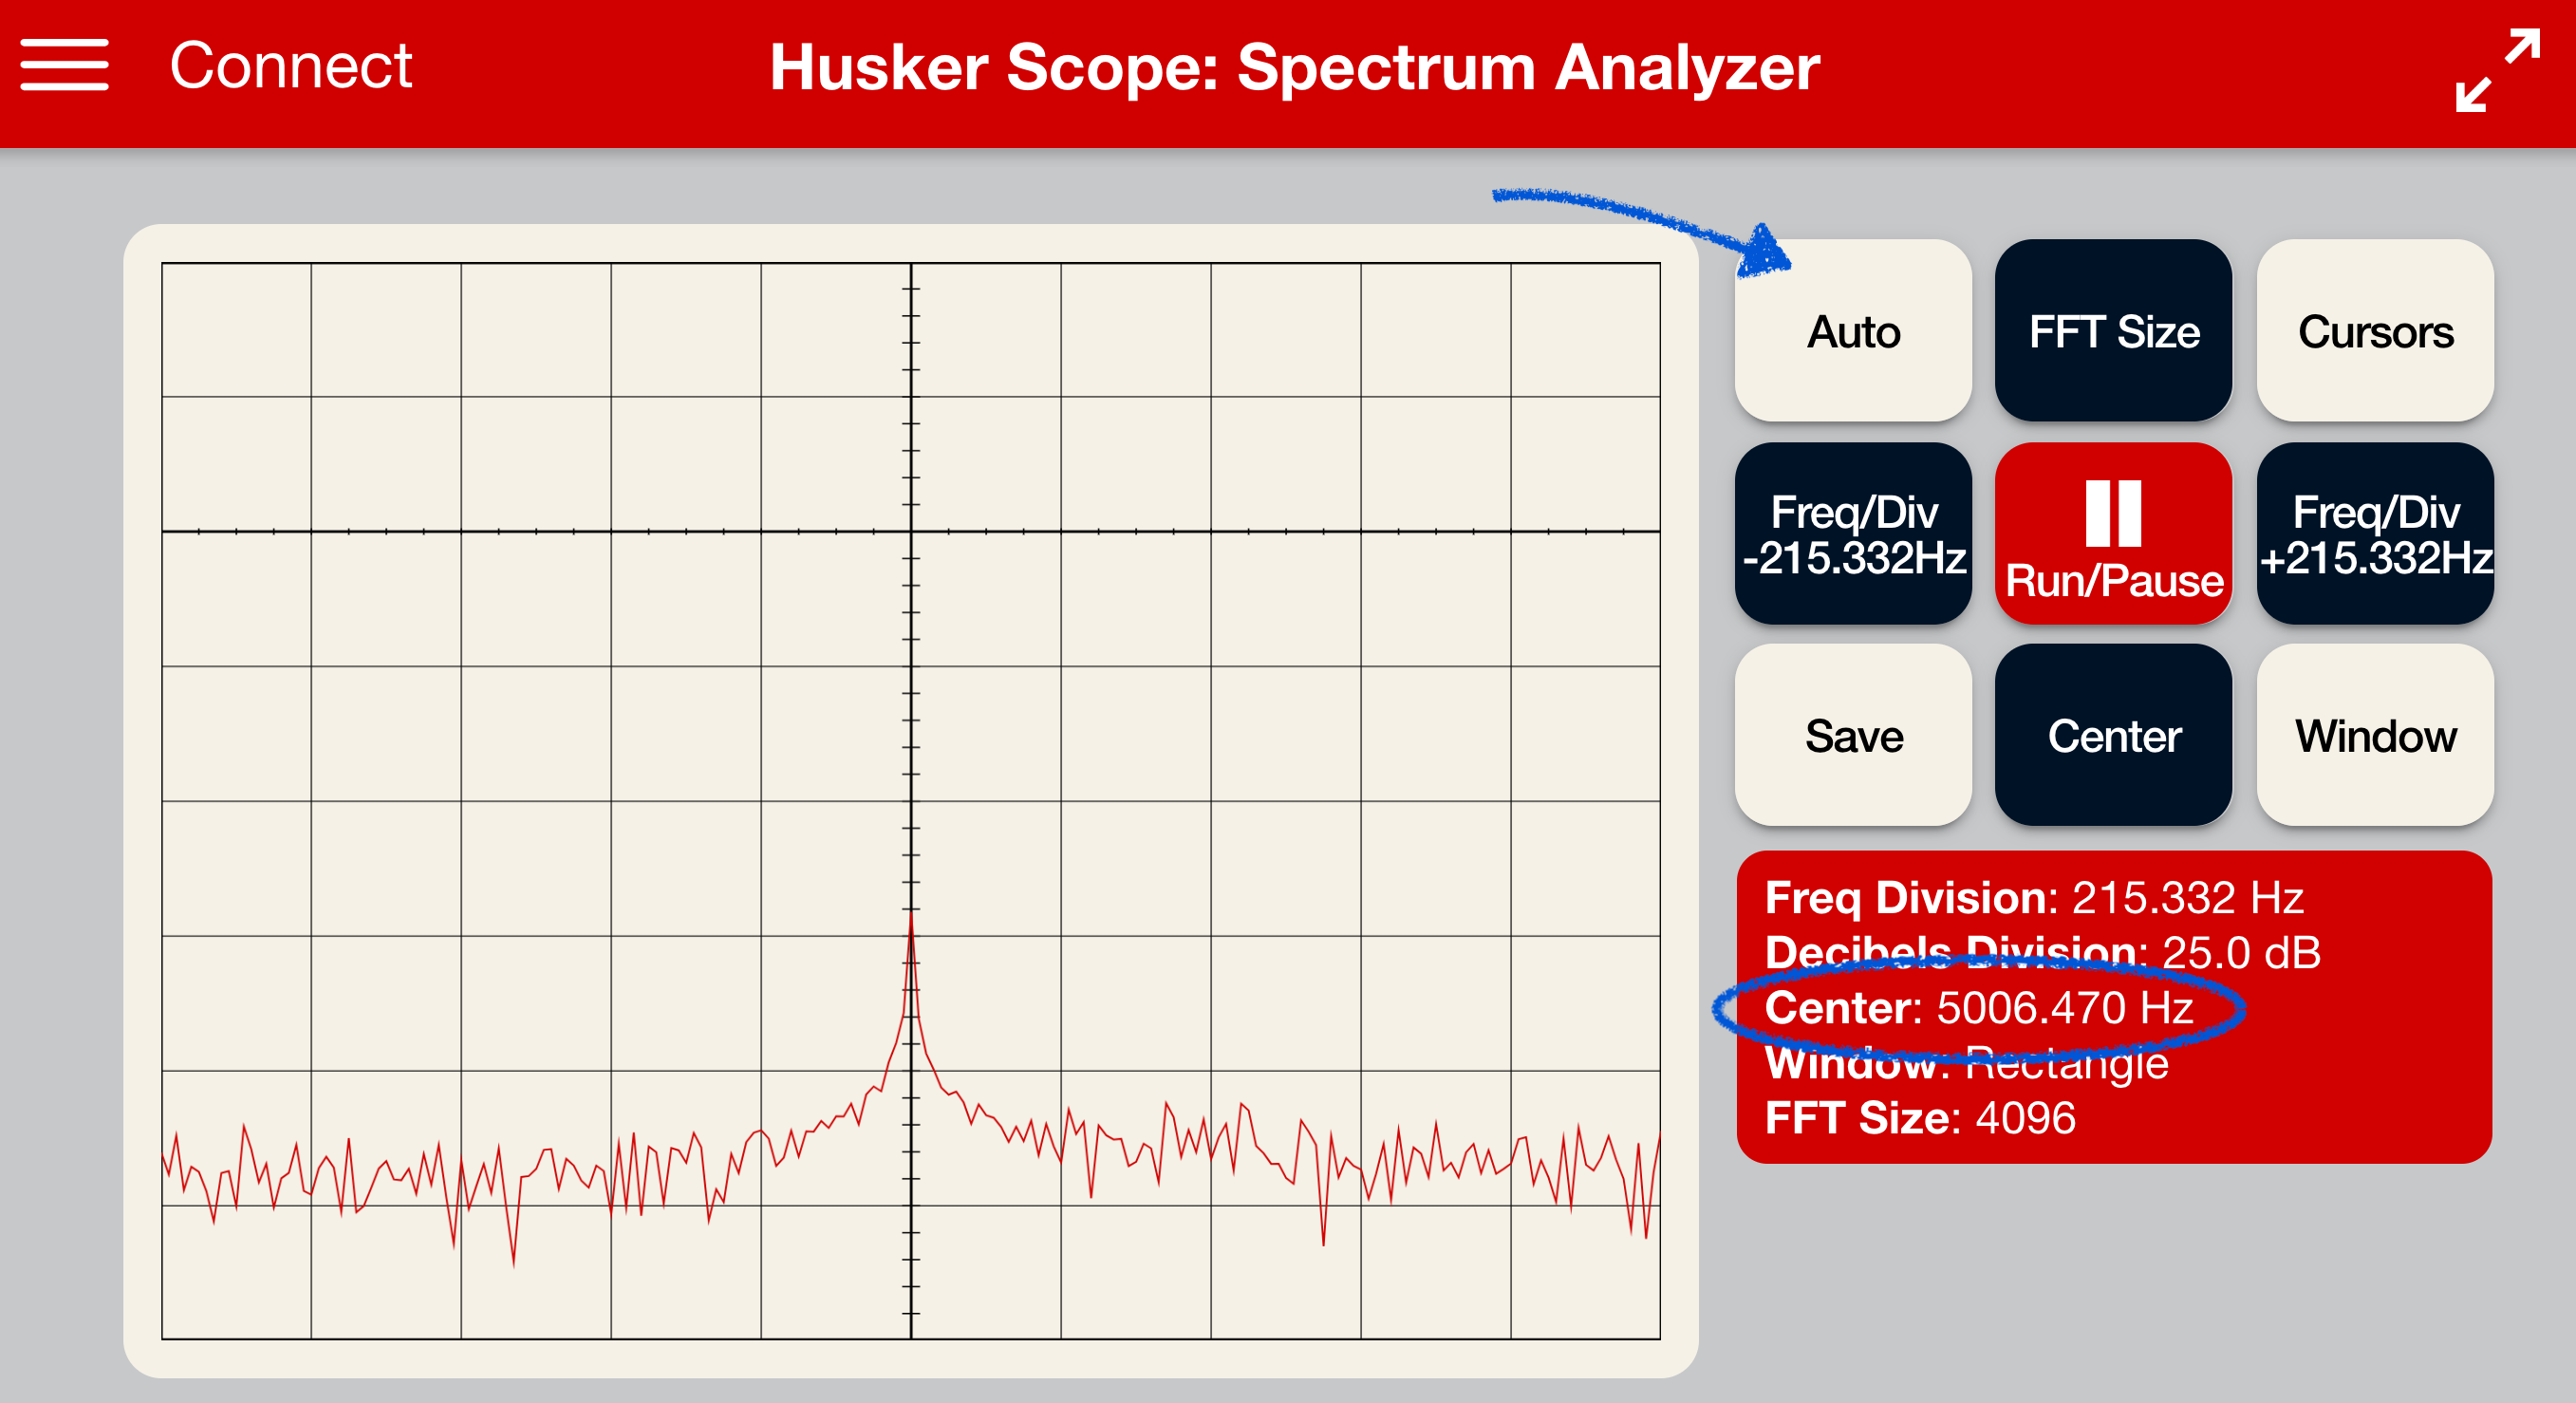
\includegraphics[width=10cm]{SpectrumAnalyzer}
    \caption{Spectrum Analyzer showing a peak near 5kHz \label{fig:spectrumAnalyzer}}
\end{figure}

After your code generates the correct tone, add code so that the continuous tone is generated only when the system is in Continuous Tone mode (Requirements~\ref{spec:modes} \& \ref{spec:continuousTone}).


\subsection{Single-Pulse Operation} \label{subsec:soundSinglePulseOperation}

A fully-correct implementation of Single-Pulse Operation mode has the alarm chirp only if an object is detected closer than the threshold range (Requirement~\ref{spec:singlePulseOperation}).
If you and your partner are working synchronously together -- if you have a working distance sensor -- then temporarily comment-out the code in \function{manage_sensor()} that initiates an ultrasonic pulse.
For the purposes of getting your alarm to chirp, you are temporarily going to have the alarm chirp whenever the pushbutton is pressed.

\vspace{.5cm}

Add another variable that counts the number of times the ISR has been triggered since the start of an alarm.
Add code to increment that counter each time the ISR runs.
You will actually use this variable as a measure of time for the alarm -- if the counter's value is $n$, then there have been $100n$~milliseconds since the start of an alarm.
Since the \lstinline{total_period} variable in the starter code is the amount of time \textit{between} alarms when the system is in Normal Operations mode, add code to reset the counter to 0 when it reaches \lstinline{total_period}. %this, perhaps, belongs in the integration piece

Add another variable that indicates that an alarm should be sounded.

For now, add code that, whenever a ping is requested (see Section~\ref{subsec:readPushbutton}):
\begin{itemize}
    \item The variable indicating that an alarm should be sounded becomes \lstinline{true}
    \item The variable that counts the number of times the ISR has been triggered becomes 0
    \item The variable indicating that a ping is requested becomes \lstinline{false}
\end{itemize}

Recall that the \lstinline{on_period} variable is used to determine how long to generate a tone (and illuminate the LEDs) after detecting an object.
(Since you don't yet have a working distance sensor, you're temporarily choosing to generate a tone whenever the user requests a ping.)
You can now introduce code that will generate the tone whenever these two things are true: an alarm should be sounded, and when the counter is less than \lstinline{on_period}.

Since the piezo should only chirp once, add code to set the ``alarm should be sounded'' variable to \lstinline{false} when the counter exceeds \lstinline{on_period}.

\vspace{.5cm}

Test your code.

\vspace{.5cm}

You may have noticed that when you press the pushbutton, the piezodisc generates a tone for considerably longer than 50ms -- it can hardly be described as a ``chirp.''
Change the value assigned to \lstinline{on_period} to the value that will correctly have the tone generated for only 50ms.

\ifbool{offerdecompositionhints}{
    \paragraph{Hint} What is $50ms \div 100\mu s$?
}{} \\

Now add code to illuminate both LEDs for the same 50ms that the piezodisc generates a tone and then deluminates the LEDs just as the tone is silenced.

\vspace{.5cm}

Most of the object detection work for Single-Pulse Operation takes place in Section~\ref{subsec:distanceSinglePulseOperation}.
You will finish implementing Single-Pulse Operation in Section~\ref{subsec:integrationSpeedSinglePulseOperation} by integrating the detection code from Section~\ref{subsec:distanceSinglePulseOperation} with the alarm code from Section~\ref{subsec:soundSinglePulseOperation}.
This will require small changes to the code.
